% Shared preamble for the CIG-AMF formal-research papers.
% IEEEtran conference class; compiles on Overleaf without modification.
\documentclass[conference]{IEEEtran}
\IEEEoverridecommandlockouts

\usepackage{cite}
\usepackage{amsmath,amssymb,amsfonts}
\usepackage{amsthm}
\usepackage{algorithm}
\usepackage{algorithmic}
\usepackage{graphicx}
\usepackage{textcomp}
\usepackage{xcolor}
\usepackage{booktabs}
\usepackage{url}
\usepackage[hidelinks]{hyperref}

\def\BibTeX{{\rm B\kern-.05em{\sc i\kern-.025em b}\kern-.08em T\kern-.1667em\lower.7ex\hbox{E}\kern-.125emX}}

\newtheorem{theorem}{Theorem}
\newtheorem{lemma}[theorem]{Lemma}
\newtheorem{proposition}[theorem]{Proposition}
\newtheorem{corollary}[theorem]{Corollary}
\theoremstyle{definition}
\newtheorem{definition}[theorem]{Definition}
\newtheorem{remark}[theorem]{Remark}
\newtheorem{example}[theorem]{Example}

% A machine-checked statement carries its Lean declaration name.
\newcommand{\lean}[1]{\textsf{\footnotesize #1}}
\newcommand{\leanbox}[1]{%
  \par\vspace{2pt}\noindent
  {\footnotesize\textsf{Lean: #1}}\par\vspace{2pt}}

% Evidence classes, used consistently and never interchangeably.
\newcommand{\PROVED}{\textsc{proved}}
\newcommand{\CERT}{\textsc{certificate}}
\newcommand{\NUM}{\textsc{numerical}}
\graphicspath{{../_figures/}}


\begin{document}

\title{Exact Alternatives and the Price of\\Surrogate Certification
in Support-Aware Compression}

\author{\IEEEauthorblockN{Vu Phan An Nguyen}
\IEEEauthorblockA{\textit{Rider University} \\
Lawrenceville, NJ, USA}}

\maketitle

\begin{abstract}
A compression is chosen by comparing losses, and a learner that must choose one under noise
faces an information game whose alternative set is the collection of worlds in which the
choice would be wrong. That set is usually replaced by a surrogate: the extrema realising
each loss are frozen at their current positions, and only they are allowed to move. We show
the surrogate is wrong in both directions and that the error is unbounded. First we pin the
alternative set exactly: with a linear world model the loss is half the oscillation of
finitely many linear forms, and the set of worlds making a retained set $\varepsilon$-wrong
is \emph{equal} to a finite union of polyhedron-intersect-halfspace pieces---an equality
proved in both directions, with the strict inequality handled by an explicit modulus rather
than silently closed. Second we certify: a primal point with multipliers proves a regional
minimum for every feasible competitor, and a prior on alternatives whose averaged per-query
information is dominated by the query cost bounds \emph{every} admissible design, not a
parametric family. Third we measure. On one family the frozen surrogate overprices the
information, with ratio bounded by $16/M$ and observed at $0.0156$; on another it underprices
it, with ratio at least $(M+3)/24$ and observed at $64.6$. No constant-factor guarantee
relating the two is possible. Separately, certifying the Top-$C$ margin costs up to three
orders of magnitude more than making the decision the margin justifies, and beyond a
threshold the certificate is unattainable at any cost while the decision remains settled. We
state this as an information-rate separation, not a sample-count ratio: the deterministic
chain converting the two is complete, but its one probabilistic input --- a per-step
confidence guarantee for the algorithm's own statistic --- is not yet instantiated.
\end{abstract}

\begin{IEEEkeywords}
compression, alternative sets, experimental design, convex certificates, formal verification
\end{IEEEkeywords}

\section{Introduction}
\label{sec:intro}

\subsection{The question}

Let a world be $\theta$, let $T$ index a retained coordinate set, and let $L_{\theta,K}(T)$
be the compression loss of $T$ measured on the deployment support $K$. The learner must
return a $T$ whose regret is at most $\varepsilon$, and it pays for observations. Its cost
is governed by an information game whose inner infimum ranges over the \emph{alternatives}:
the worlds in which the returned $T$ would be wrong.

Computing that infimum requires knowing the alternative set. The natural shortcut is to
freeze the argmax and argmin realising each loss and ask how far the observations must move
to reverse the comparison. This paper is about how badly that shortcut misprices the game,
and about what it takes to replace it with something certified.

\subsection{What is new, against the nearest sources}

Information games with several correct answers, and alternative sets that decompose into
finitely many convex regions, are developed in the literature; Degenne and
Koolen~\cite{degenne2019} for the multiple-answer setting, and Wang and
You~\cite{wangyou2026} for the piecewise-convex decomposition. We take that structure as
given and do not claim it. We also do not overstate it: \cite{wangyou2026} leaves an exact
stopping threshold problem-dependent and labels part of its scaling argument heuristic, so
it should not be cited as having closed the algorithmic question.

Bennouna et al.~\cite{bennouna2026} study data informativeness in linear optimisation. That
is the closest work on ``which observations matter for a decision'', and its scope is linear
optimisation; we do not extend its statements to noisy compression, which it does not make.

Three things here are ours.
\begin{enumerate}
\item[1)] \textbf{An equality, not a decomposition found by search.} We prove the
alternative set \emph{equals} the union of its regions, and we handle the strict inequality
with an explicit modulus, including the case in which the strict part is empty and the
region must be dropped rather than closed.
\item[2)] \textbf{Certificates at both levels.} A KKT certificate for each region, and a
dual over the \emph{whole} query set for the design---so ``optimal'' is not shorthand for
``optimal within the family we searched''.
\item[3)] \textbf{Two-sided failure of the frozen surrogate}, with explicit families and
rates in both directions, so no constant-factor repair is possible.
\end{enumerate}

\section{The model}
\label{sec:model}

Parametrise the world linearly, $F_{\theta}(x)=\phi(x)^{\top}\theta$ on a finite domain $X$
with a fixed reference and a deployment support $K\subseteq X$. With the reference fixed the
product responses are linear in $\theta$, so for a retained set $T$ the residual at a support
point is a linear form, $r_{\theta,T}(x)=a_{T}(x)^{\top}\theta$, and
\begin{equation}
L_{\theta,K}(T)=\tfrac12\Bigl[\max_{x\in K}a_{T}(x)^{\top}\theta-\min_{x\in K}a_{T}(x)^{\top}\theta\Bigr].
\label{eq:loss}
\end{equation}
Observations are Gaussian and linear in $\theta$: query $e$ returns $Y_{e}\sim N(M_{e}\theta,\sigma_{e}^{2})$
at cost $c_{e}$, and a design is a non-negative allocation $w$ with $\sum_{e}c_{e}w_{e}=1$.

\TODOPAR{Two bridges are asserted by fixing the model rather than derived: that $a_{T}$ is
the corpus residual, and that \eqref{eq:loss} is the compression loss the corpus computes.
Both are routine but neither is proved, and the final version must either prove them or say
plainly that the model is the object of study. Do not describe the reduction as derived.}

\section{The alternative set, exactly}
\label{sec:alt}

\subsection{The equality}

Fix $T$ and a competitor $S$. Pinning which support points realise the four extrema cuts out
a polyhedron, and on it the doubled loss difference is a single linear form.

\begin{theorem}[Region form]
\label{thm:region}
If $x,y$ realise the max and min of $r_{\theta,T}$ and $p,q$ those of $r_{\theta,S}$, then
\begin{equation}
2\bigl[L_{\theta,K}(T)-L_{\theta,K}(S)\bigr]
= \bigl(a_{T}(x)-a_{T}(y)-a_{S}(p)+a_{S}(q)\bigr)^{\top}\theta .
\label{eq:regionform}
\end{equation}
\end{theorem}

\leanbox{\lean{loss\_eq\_of\_extrema}, \lean{region\_form\_is\_linear} in
\lean{LeanPaperAAlternativesV1}}

\begin{theorem}[The alternative set is the union]
\label{thm:alteq}
$L_{\theta,K}(T)-L_{\theta,K}(S)>\varepsilon$ holds if and only if there exist extrema
indices satisfying the region conditions and making the linear form
of~\eqref{eq:regionform} exceed $2\varepsilon$.
\end{theorem}

\leanbox{\lean{alt\_iff\_exists\_region}, with \lean{exists\_extrema}, in
\lean{LeanPaperAAlternativesV1}}

Both directions matter. Left to right says the true extrema always pin \emph{some} region,
so the union is complete; right to left says every piece consists of genuine alternatives,
so nothing spurious is added. Neither is a search result.

\subsection{The closure, where care is needed}

The alternative condition is strict, and an infimum over a strict region is not in general
the infimum over its closure. The exchange is legitimate exactly when the region contains a
strictly bad point.

\begin{theorem}[Closure exchange]
\label{thm:closure}
If the region is convex and contains $\theta_{+}$ with $v^{\top}\theta_{+}>c$, then the
infimum of the energy over $\{v^{\top}\theta>c\}$ equals its infimum over
$\{v^{\top}\theta\ge c\}$.
\end{theorem}

\leanbox{\lean{strict\_inf\_eq\_closed\_inf}, with \lean{segment\_stays\_strict} and
\lean{energy\_segment\_bound}, in \lean{LeanPaperAAlternativesV1}}

The proof needs no limiting argument: along the segment from a closed point towards
$\theta_{+}$ the energy moves by at most $t$ times an explicit constant, and the segment is
strictly bad for every $t>0$. When the strict part is \emph{empty} the region contributes no
alternative and must be dropped; closing it would manufacture an alternative out of a tie.

\leanbox{\lean{strict\_empty\_has\_no\_alternatives} in the same module}

\section{Certifying, at both levels}
\label{sec:cert}

\subsection{Each region}

\begin{theorem}[KKT certificate]
\label{thm:kkt}
Let $H$ be symmetric positive semidefinite and let $\lambda$ be feasible for $A\lambda\le b$
with multipliers $y\ge0$ satisfying $H(\lambda-\theta)+A^{\top}y=0$ and complementary
slackness. Then $\lambda$ minimises $\tfrac12(\cdot-\theta)^{\top}H(\cdot-\theta)$ over the
region, against every feasible competitor.
\end{theorem}

\leanbox{\lean{kkt\_region\_minimum}, with \lean{quad\_expand}, in
\lean{LeanPaperAOracleCertificateV1}}

$H$ is \emph{not} assumed invertible. That matters: a design leaving a direction unmeasured
produces a singular $H$, and a statement requiring invertibility would silently exclude the
designs one most wants to compare.

\subsection{Every design}

\begin{theorem}[Design optimality over the whole query set]
\label{thm:dual}
Let $\nu$ be a prior on alternatives with $\sum_{\ell}\nu_{\ell}=1$, $\nu\ge0$. If
$\sum_{\ell}\nu_{\ell}d_{e}(\theta,\lambda_{\ell})\le Vc_{e}$ for \emph{every} admissible
query $e$, then $J_{T}(w,\theta)\le V$ for every design $w$ with
$\sum_{e}c_{e}w_{e}=1$. With a primal allocation attaining $V$, $\sup_{w}J_{T}(w,\theta)=V$.
\end{theorem}

\leanbox{\lean{design\_upper\_bound\_of\_dual}, \lean{design\_value\_eq\_of\_primal\_dual} in
\lean{LeanPaperAOracleCertificateV1}}

This is the step that converts ``best in the family we parametrised'' into ``best''. If a
query violates the dual inequality, that violation is a direction of improvement: add the
query and re-solve.

\section{The frozen surrogate misprices, both ways}
\label{sec:proxy}

\subsection{Two families}

Let $M$ be the effective variance of one designated cheap cell; all others have variance
one, and the decision compares $\mathrm{range}(A)$ with $\mathrm{range}(B)$.

\emph{Family 1, the surrogate prices too high.} $A=(0,1,\tfrac12)$, $B=(0,\tfrac34,\tfrac12)$
with variance $M$ on $B$'s middle cell. Freezing the extrema forces four unit-variance cells
to close a gap of $\tfrac14$, giving $J_{\rm frozen}=\tfrac1{128}$. The true alternative may
instead lift $B$'s middle cell to become the new maximum, at cost $1/8M$, so
\begin{equation}
J_{\rm full}/J_{\rm frozen}\le 16/M\longrightarrow0 .
\label{eq:fam1}
\end{equation}

\emph{Family 2, the surrogate prices too low.} $A=(0,1,\tfrac34)$, $B=(0,\tfrac12,\tfrac14)$
with variance $M$ on $A$'s maximum, so $J_{\rm frozen}=1/8(M+3)$. Lowering the cheap maximum
is not enough because the runner-up at $\tfrac34$ remains; the true cost stays bounded below
and
\begin{equation}
J_{\rm full}/J_{\rm frozen}\ \ge\ (M+3)/24\longrightarrow\infty .
\label{eq:fam2}
\end{equation}

\subsection{Computed, with every region certified}

A word on what $J_{\rm frozen}$ is, because the ratios are only coherent under the right
reading. $J_{\rm frozen}$ is the \emph{frozen-linear} surrogate: the range comparison is
linearised at the current extrema and the ordering conditions are dropped. It is \emph{not}
the minimum over the region that pins those extrema. Were it that, a region being a subset
of parameter space would force $J_{\rm full}\le J_{\rm region}$ and a ratio above one would
be impossible. Family~2's ratios exceed one because the surrogate optimises over a set that
is \emph{not} contained in the true alternative set: it admits parameters violating the
ordering conditions, which are not alternatives at all. Neither set contains the other, and
that is precisely why the surrogate can err in both directions.

\begin{table}[t]
\caption{The frozen surrogate against the true oracle. Each cell solves all $81$ regions and
every one of them carries a KKT certificate, not only the winner. \NUM{}}
\label{tab:proxy}
\centering
\footnotesize
\begin{tabular}{@{}rrrrr@{}}
\toprule
$M$ & Fam.\,1 ratio & $16/M$ & Fam.\,2 ratio & $(M{+}3)/24$ \\
\midrule
$1$ & $1.000$ & $16$ & $1.000$ & $0.167$ \\
$64$ & $0.2388$ & $0.25$ & $4.59$ & $2.79$ \\
$256$ & $0.0618$ & $0.0625$ & $16.58$ & $10.79$ \\
$1024$ & $0.0156$ & $0.0156$ & $64.58$ & $42.79$ \\
\bottomrule
\end{tabular}
\end{table}

Two features deserve emphasis. The surrogate is \emph{exact} at small $M$ and only breaks
past a threshold, so the failure is a genuine transition rather than a modelling artefact.
And because the error runs in both directions on the same decision rule, no constant-factor
guarantee relating $J_{\rm frozen}$ to $J_{\rm full}$ can exist.

\TODOPAR{These two families are stated for an oracle over cell ranges with per-cell
observations. Realising them inside the model of Section~\ref{sec:model}---an explicit
$F_{\theta}$, reference and admissible queries---has \emph{not} been done. If the move from
per-cell to per-response observation changes the Hessian, the energies must be recomputed;
the constants above must not be transported by assertion. This is the first thing the final
version owes.}

\section{Certifying a margin costs more than deciding}
\label{sec:margin}

On the full cube take $F(x_{1},x_{2})=ax_{1}+bx_{2}+cx_{1}x_{2}$ with $a>b>0$, $c>0$ and a
corner reference. Then $L(\{1\})=(b+c)/2$ and $L(\{2\})=(a+c)/2$, so the \emph{decision} is
settled by the sign of $a-b$ alone, while the interaction bound is $\delta_{I}=c$ and the
Top-$C$ margin \emph{certificate} $\rho\ge2\delta_{I}$ reads $a-b\ge2c$. Both are half-space
questions about $\theta$, but about different half-spaces.

\begin{table}[t]
\caption{Cost of the margin certificate against the decision it justifies, at $a=3$, $b=1$,
$\varepsilon=0.1$. \NUM{}}
\label{tab:margin}
\centering
\footnotesize
\begin{tabular}{@{}rrrr@{}}
\toprule
$c$ & $\Gamma_{\rm dec}$ & $\Gamma_{\rm cert}$ & ratio \\
\midrule
$0.25$ & $0.6050$ & $0.0313$ & $19.4$ \\
$0.75$ & $0.6050$ & $0.0035$ & $174.2$ \\
$0.90$ & $0.6050$ & $0.0006$ & $1089.0$ \\
$\ge1.00$ & $0.6050$ & $0$ & $\infty$ \\
\bottomrule
\end{tabular}
\end{table}

\begin{theorem}[Certifying is never cheaper]
\label{thm:cert}
If every world satisfying the certificate condition is one in which $T$ is safe, then the
decision's alternatives are contained in the certificate's, so
$\Gamma_{\rm cert}\le\Gamma_{\rm dec}$.
\end{theorem}

\leanbox{\lean{certification\_costs\_at\_least\_as\_much} in
\lean{LeanPaperAOracleCertificateV1}}

At $a-b\le2c$ the true world itself fails the margin condition, so the certificate is
unattainable at any cost while the decision remains settled.

\NOTEPAR{Two scope limits. This is an \emph{information-rate} separation, not a ratio of
expected sample counts: without a matching stopping theorem the two are not interchangeable.
And the lower bound is against \emph{this} certificate, the one the corpus uses; a weaker
sufficient condition tailored to the family might close much of the gap, and no claim is made
about ``every certificate''.}

\section{No constant-factor guarantee, after the allocation is optimised}
\label{sec:separation}

The mispricing above is at a fixed design. The question a practitioner asks is whether it
survives choosing the design well, so the statement below is about the games
\[
\Gamma_{\bullet}(\theta)\;=\;\sup_{w\in\Delta}\ \inf_{\lambda\in\mathrm{Alt}_{\bullet}
\cap\,\Theta_{0}}\ \tfrac12\sum_{e}\frac{w_{e}(\lambda_{e}-\theta_{e})^{2}}{\nu_{e}},
\]
with $\mathrm{Alt}_{\rm true}$ the worlds in which retaining $A$ is strictly worse and
$\mathrm{Alt}_{\rm proxy}$ the worlds satisfying the frozen contrast.

\paragraph{The model class, and why the tables must be centred.}
$\Theta_{0}$ is the centred class: each arm's table sums to zero. That is not decoration.
On the centred class the product response \emph{is} the table, with no additive remainder,
so the energy above is the information the queries carry rather than a stand-in for it. The
tables as printed are not centred, so a statement naming the raw cell values and asserting
$\theta\in\Theta_{0}$ has contradictory hypotheses and says nothing. An earlier version of
our wrapper did exactly that. The repair is to subtract each arm's mean and to prove that
this changes nothing the decision can see: a common shift of an arm moves neither its range,
nor the frozen contrast, nor---when the world and the candidate are shifted together---the
energy. The worlds used below are therefore
\[
\theta^{-}=\bigl(-\tfrac12,\tfrac12,0,0;\ -\tfrac7{16},\tfrac5{16},\tfrac1{16},
\tfrac1{16}\bigr),\quad
\theta^{+}=\bigl(-\tfrac9{16},\tfrac7{16},\tfrac3{16},-\tfrac1{16};\
-\tfrac14,\tfrac14,0,0\bigr),
\]
which are the paper's two tables, centred, and which lie in $\Theta_{0}$.

\leanbox{\lean{shiftArms}, \lean{rng\_sub\_const}, \lean{energy\_shiftArms},
\lean{inClass\_center}, \lean{thetaLowC\_eq\_centered\_raw},
\lean{low\_world\_hypotheses\_consistent} in \lean{LeanPaperASeparationV1}}

\begin{theorem}[The surrogate is wrong in both directions, at worlds that exist]
\label{thm:sep}
Put variance $M$ on the two cells named by each family and $1$ elsewhere. At $\theta^{-}$,
$\Gamma_{\rm true}/\Gamma_{\rm proxy}\le64/M$; at $\theta^{+}$,
$\Gamma_{\rm true}/\Gamma_{\rm proxy}\ge M/96$. Consequently, for every $c>0$ there is a
single $M$ at which the first ratio falls below $c$ and the second rises above it, so no
constant relates the surrogate to the truth in both families at once.
\end{theorem}

Both games are suprema of infima, so the statement is empty unless they exist. They do: each
inner set is nonempty and bounded below by zero, and each outer set is capped by the cheap
alternative the separation already exhibits, so an explicit bound is available in each of
the four cases.

\leanbox{\lean{low\_separation\_at\_world}, \lean{high\_separation\_at\_world},
\lean{exists\_low\_games}, \lean{exists\_high\_games},
\lean{no\_constant\_factor\_on\_families} in \lean{LeanPaperASeparationV1}}

\NOTEPAR{Scope. $M$ is a known variance of the observation model, so this is a separation
within a heteroscedastic family, at $\varepsilon=0$, at an instance whose decision is
unique. Removing the dependence on heteroscedasticity needs the $r$-pair variant, which is
not proved.}

\paragraph{What is and is not new here.}
That an information proxy can select a design lacking identifiability is
known: Overstall studies expected Fisher-information gain and gives conditions under
which the optimal design induces non-identifiability~\cite{overstall2022}. That an
acquisition rule should target the decision rather than the predictor is
known~\cite{filstroff2021}, as is error amplification under model
misspecification~\cite{tang2026}, and decision-focused sequential design already carries
a sample-complexity guarantee together with an instance on which a prediction-focused
method fails to eliminate a decision-relevant hypothesis~\cite{wan2026}. When a proxy
\emph{suffices} for a decision, and what to do when it does not, is itself a studied
question~\cite{schutte2026}, and targeted active learning for probabilistic models already
carries label-complexity bounds~\cite{tosh2022}. In combinatorial
complexity there is now a total Boolean function with
$R(f)=\widetilde{O}(\sqrt{C(f)})$~\cite{bendavid2026}, which forecloses the generic
headline that certification must cost more than deciding.

So the generic statements are taken. What this paper claims is narrower and, we think,
sharper: the \emph{observation model is correct}, the stopping certificate is
\emph{valid}, and the decision objective is \emph{unchanged}; the only thing altered is
the geometry used to score allocations, and that alone changes what the design can learn.
The failure is not misspecification and not an invalid test --- it is a frozen extremum
in an otherwise correct model.

\subsection{A repair criterion, and exactly what it does not do}

A design carries a certificate when a computable barrier separates the surrogate's value
from the nearest switch,
\[
J_{\rm proxy}(w)<B_{\rm switch}(w)\ \Longrightarrow\ J_{\rm true}(w)=J_{\rm proxy}(w),
\]
which is a theorem. What it is worth is a separate question, and answering it requires
care about the denominator.

Wherever the certificate fires it forces $J_{\rm true}=J_{\rm proxy}$, so a certified
design inherits the separation:
\begin{equation}
\mathrm{Cert}(w)\ \Longrightarrow\ \frac{J_{\rm proxy}(w)}{\Gamma_{\rm proxy}}\;\le\;
\frac{64}{M}.
\label{eq:certceiling}
\end{equation}
It is tempting to read \eqref{eq:certceiling} as saying certified designs become worthless
as $M$ grows. That reading is wrong, and the reason is that $\Gamma_{\rm proxy}$ is the
wrong yardstick: what a repair is for is the \emph{true} game, so the quantity to bound is
$J_{\rm true}(w)/\Gamma_{\rm true}$, and at the optimum level
\[
\frac{\Gamma_{\rm cert}}{\Gamma_{\rm true}},
\qquad
\Gamma_{\rm cert}=\sup_{w\,:\,\mathrm{Cert}(w)}J_{\rm true}(w).
\]
Converting \eqref{eq:certceiling} into those units costs the separation back,
$J_{\rm true}(w)/\Gamma_{\rm true}\le(64/M)\,\Gamma_{\rm proxy}/\Gamma_{\rm true}$, and on
the sweep's own bracket that product is $66.2$, $18.4$, $6.43$, $3.42$ and $2.58$ at
$M=1,4,16,64,256$. It exceeds one at every size: \textbf{in true units the ceiling is
vacuous, and \eqref{eq:certceiling} constrains the repair's efficiency not at all.}
\CERT{}

The same correction applies to the exhibited witness. At $M=256$ the rational design
$w=\tfrac1{1000}(1,1,1,1,1,1,497,497)$ has $J_{\rm proxy}=1/128\,000$ and $B_{\rm
switch}=497/24\,096\,000$, so $J_{\rm proxy}<B_{\rm switch}$ and the criterion
\emph{fires}. That design is $0.402\%$ of the floored surrogate optimum but $4.15\%$ of the
bracketed true optimum --- a factor of ten between the two readings, and the second is the
one that matters. One poor witness is in any case not a statement about
$\Gamma_{\rm cert}$: at $M=256$ none of the $43$ sampled designs is certified, so this
sweep exhibits no certified design other than the witness and gives no lower bound on
$\Gamma_{\rm cert}$ at all.

\NOTEPAR{So the honest position on repair is neither positive nor negative: it is
undetermined. What the criterion gives is a \emph{verified} equality at the designs where
it fires; what is not known is the value of $\Gamma_{\rm cert}/\Gamma_{\rm true}$, because
\eqref{eq:certceiling} is vacuous in true units and the sweep certifies too few designs to
estimate the supremum. Settling it means optimising $J_{\rm true}$ \emph{over the
certificate region}, with $\Gamma_{\rm true}$ as denominator. Do not write that certified
designs are worthless, and do not write that the criterion repairs the surrogate.}

\leanbox{\lean{barrier\_implies\_equality}, \lean{optima\_equal\_of\_certificate},
\lean{certifiable\_fraction\_le\_sixtyfour\_over\_M},
\lean{design\_certificate\_insufficient} in \lean{LeanPaperARepairV1}}

\subsection{A learner that stops under a certificate}
\label{sec:learner}

The separation is about information rates. Turning one into a sample count needs a rule that
actually stops, so we run one: a learner that sees only counts, observations and known
variances, brackets each answer's value by cutting planes at the current estimate, keeps the
answers whose upper bracket survives $\max_{S}l_{S}-2Lr_{t}$, tracks the selected answer's
design with forced exploration, and stops when a \emph{certified lower} bound on every
region's infimum exceeds the threshold. The certificate is weak duality,
$g(y)=-\tfrac12y^{\top}AH^{-1}A^{\top}y+y^{\top}(A\hat\mu-b)\le\min$ for every $y\ge0$, so
it is valid whatever the optimiser does; a primal objective is an \emph{upper} bound and
cannot justify stopping.

\NOTEPAR{These numbers are from the \emph{pre-damping} policy and must not be read as
measuring the algorithm described above. The bracket was subsequently corrected --- running
minimum of the relaxation values, damped cutting-plane step, regional dual solved to
tolerance --- together with a feasibility check on primal witnesses and a conservative
slack in the selection rule. All of those change the allocation, so the $144$ runs below
measure a different policy. The artifact is tagged \texttt{policy\_generation:
pre-damping} and \texttt{do\_not\_combine}; the replacement run under the corrected
policy is reported separately and these figures are to be replaced by it, not averaged
with it.}

On a centred instance with $M=16$, over $12$ runs at each of
$\alpha\in\{0.1,0.05,0.02,0.01\}$: every one of the $144$ stopped runs across all three arms
returned the correct answer with zero regret, none was censored, and mean stopping times were
$1741\pm74$ (learner), $1156\pm43$ (oracle diagnostic) and $1617\pm58$ (uniform). The
asymptotic benchmark is the bracket $1/\Gamma_{\rm comp}\in[43.00,43.00]$, its lower side
from an achieved design and its upper side from a prior $p$ over the collected alternatives
with $\max_{e}(\sum_{\ell}p_{\ell}g_{\ell})_{e}$ recomputed from $p$.

\paragraph{What the implementation guarantees, and how that is checked.}
Three properties the analysis needs are enforced in the code and checked structurally
rather than asserted. The oracle's own error must vanish for any accumulation argument to
apply, so the cutting-plane tolerance is tightened as $1/n^{2}$ --- floored at a width the
bracket can actually reach, since a tolerance it cannot clear never fires the early break
--- and the iteration budget
raised with the refresh index, and the achieved bracket gap is recorded at every refresh
and checked to decrease --- an iteration cap alone guarantees nothing. Every refresh is
stored and the stored count is checked against the number performed, so no trace is
silently truncated. And the learner cannot read the true world because the world is not
in scope: \texttt{run} receives a sampler closure, \texttt{theta} is not among its
parameters, and the self-check inspects the signature instead of promising it in a
comment. \CERT{}

\NOTEPAR{Read this as what it is. The three means are \emph{measurements} at finite
$\alpha$, not a confirmation of a predicted ordering: the learner is not faster than uniform
here, and the differences are within a few standard errors. The gap is the price of
learning the allocation and of the oracle calls, and asymptotic optimality does not excuse
it. The oracle arm reads the true
world and is a diagnostic, not a competitor. No selection snapshot ever narrowed the answer
set---not even on the swapped world whose correct answer is second in the tie-break
order---so these runs are evidence about \emph{stopping}, not about elimination. Say that,
and do not write ``the learner attains $\Gamma_{\rm comp}$''.}

\subsection{The confidence sequence, with Ville proved}
\label{sec:ville}

The stopping rule is correct if the statistic crossing its threshold is unlikely under the
true world, and that reduces to one inequality: a non-negative supermartingale started at
mean one exceeds $1/\delta$ with probability at most $\delta$. Mathlib has Doob's maximal
inequality for non-negative \emph{sub}martingales, which is the wrong direction, and does
not have Ville's. We prove it, from optional stopping:

\begin{theorem}[Ville, at a finite horizon]
\label{thm:ville}
Let $M$ be a non-negative supermartingale. Then for every $\lambda>0$ and every $N$,
\[
\lambda\cdot\Pr\Bigl(\exists\, j\le N:\ M_{j}\ge\lambda\Bigr)\ \le\ \mathbb{E}[M_{0}].
\]
\end{theorem}

The proof is three steps. Negating $M$ gives a submartingale, so optional stopping between
the constant time $0$ and the hitting time of $[\lambda,\infty)$ capped at $N$ gives
$\mathbb{E}[M_{\tau}]\le\mathbb{E}[M_{0}]$. On the event that $M$ reaches $\lambda$ by time
$N$ the stopped value is at least $\lambda$, and off it the value is at least $0$ because
$M$ is non-negative. Combining the two bounds the probability.

The consequence is stated for an actual measure and an actual supermartingale, with no
hypothesis standing in for Ville: if crossing the threshold forces the mixture past
$1/\delta$, the rule errs with probability at most $\delta$.

\leanbox{\lean{ville\_finite\_horizon}, \lean{confidence\_of\_supermartingale},
\lean{stopping\_error\_le} in \lean{LeanPaperA7ConfidenceV1}}

\paragraph{A process it applies to.}
A theorem about supermartingales is worth what its instances are worth, so we exhibit one.
Take $\Omega=\mathbb{N}\to\mathbb{R}$ with the law of independent $\mathcal{N}(0,1)$
observations, let $Y_{n}$ be the $n$-th observation, and let
\[
\Lambda_{n}(u)=\exp\!\bigl(uY_{n}-u^{2}/2\bigr),
\qquad
M_{t}(u)=\prod_{n\le t}\Lambda_{n}(u).
\]
The coordinates are independent because the law is a product; the increments are therefore
independent, being measurable functions of them; and $\mathbb{E}\Lambda_{n}(u)=1$ exactly,
which is the Gaussian moment generating function $\mathbb{E}e^{uY}=e^{u^{2}/2}$ cancelled
against the tilt. Independence makes the conditional expectation of the next increment its
mean, so $M(u)$ is a martingale for the natural filtration --- and Theorem~\ref{thm:ville}
applies to it, giving
$\Pr(\exists\, j\le N:\ M_{j}(u)\ge1/\delta)\le\delta$ on that stream.

\leanbox{\lean{obs\_indep}, \lean{incr\_integral}, \lean{mix\_indep\_incr},
\lean{mix\_martingale\_step}, \lean{mix\_supermartingale}, \lean{stream\_confidence} in
\lean{LeanPaperA7StreamV1}}

\NOTEPAR{Scope, exactly. The instance has a \emph{fixed} tilt $u$ and queries the same
coordinate at every step. The learner's statistic is a mixture over $u$ and its query is
chosen from the history, so this is not that process. What it establishes is that the
supermartingale hypothesis is satisfiable by a real observation model and that the Gaussian
step calculation is the right one. Carrying it across needs the predictable query to enter
the conditional expectation, and that is not done. Do not write that the anytime guarantee
is proved for the algorithm.}

\subsection{Separation without heteroscedasticity: the $r$-pair family}
\label{sec:rpair}

Theorem~\ref{thm:sep} needs $M$ to grow, so at $M=1$ it says nothing and the separation can
be read as an artefact of a badly conditioned observation model. It is not. Widen the
relation instead of the variance: give each arm $2r+2$ actions, with $r$ disjoint pairs of
middle cells in arm $B$. The frozen proxy still watches only the four anchors, while the
adversary may move whichever pair the design has measured least.

\begin{theorem}[The $r$-pair separation]
\label{thm:rpair}
With $r$ disjoint pairs and a unit design budget, some pair carries weight at most $1/r$, so
$\Gamma_{\rm true}\le1/8Mr$ while $\Gamma_{\rm proxy}\ge1/512$. Hence
$\Gamma_{\rm true}/\Gamma_{\rm proxy}\le64/rM$, and for every $c>0$ there is an $r$ at which
the ratio falls below $c$ \emph{at $M=1$}.
\end{theorem}

The pigeonhole is the whole mechanism, and it is what makes the bound hold after the
allocation has been optimised: the adversary reads $w$ and then chooses the pair.

\leanbox{\lean{exists\_light\_pair}, \lean{pair\_shift\_energy},
\lean{light\_pair\_energy\_le}, \lean{rpair\_ratio\_le},
\lean{no\_constant\_factor\_at\_unit\_variance} in \lean{LeanPaperARPairV1}}

\paragraph{The matching lower bound.}
Both sides are now proved, so the ratio is $\Theta\bigl((rM)^{-1}\bigr)$ and not merely
$O$. The lower side needs an explicit design rather than a pigeonhole: the anchor design
spreads mass over the four contrast cells and the $2r$ pair cells, and the four-square
inequality
\[
\tfrac{1}{4}<x_{1}-x_{2}+x_{3}-x_{4}
\;\Longrightarrow\;
x_{1}^{2}+x_{2}^{2}+x_{3}^{2}+x_{4}^{2}>\tfrac{1}{64}
\]
turns a range gap at the contrast into an energy floor. Evaluating $\Gamma_{\rm true}$ at
that design gives
\[
\frac{1}{128\,(4+2rM)}\;\le\;\Gamma_{\rm true}\;\le\;\frac{1}{8rM},
\qquad
\frac{2}{2+rM}\;\le\;\frac{\Gamma_{\rm true}}{\Gamma_{\rm proxy}}\;\le\;\frac{64}{rM}.
\]

\leanbox{\lean{anchorDesign}, \lean{four\_sq\_lower}, \lean{rpair\_true\_ge},
\lean{rpair\_ratio\_ge}, \lean{rpair\_theta} in \lean{LeanPaperARPairV1}}

\paragraph{The two games, as games.}
The bracket above is arithmetic about two numbers: it takes $\Gamma_{\rm true}$ and
$\Gamma_{\rm proxy}$ as given and pins their ratio. That is not yet a statement about the
$r$-pair problem, so we state it as one. Fix the world
$\theta_{0}$ with arm $A$'s anchors a unit apart and all of arm $B$ at zero, and the
variance profile unit on the anchors and $M$ on the pairs. Define
\[
\Gamma_{\rm true}
=\sup_{w\ \rm alloc}\ \inf_{\lambda:\ \mathrm{range}_{A}\lambda<\mathrm{range}_{B}\lambda}
  \mathcal{E}(w,\lambda),
\qquad
\Gamma_{\rm proxy}
=\sup_{w\ \rm alloc}\ \inf_{\lambda\in\Lambda_{\rm proxy}}\mathcal{E}(w,\lambda),
\]
where $\Lambda_{\rm proxy}$ is the set of alternatives the frozen surrogate can separate
from $\theta_{0}$ at all --- those that move an anchor and leave the pair cells alone.
Both are genuine $\sup\inf$ over the actual allocations and the actual alternatives.

\begin{theorem}[The ratio, on the games themselves]
\label{thm:rpairgames}
For $r\ge1$ and $M>0$,
\[
\frac{1}{128\,(4+2rM)}
\;\le\;\frac{\Gamma_{\rm true}}{\Gamma_{\rm proxy}}\;\le\;
\frac{16}{Mr},
\]
and all four one-sided bounds --- $\Gamma_{\rm true}\le1/(8Mr)$,
$\Gamma_{\rm true}\ge1/(128(4+2rM))$, $\Gamma_{\rm proxy}\le1$,
$\Gamma_{\rm proxy}\ge1/128$ --- are theorems, not inputs.
\end{theorem}

The proxy value stays between two absolute constants while the true value falls like
$1/(rM)$: the surrogate overstates the information available by a factor growing without
bound in $r$, at uniform variance $M=1$.

\paragraph{The same bracket, against the surrogate itself.}
$\Lambda_{\rm proxy}$ above pins the middle cells and then uses the \emph{true} ranges;
the frozen-linear surrogate pins the extremum \emph{indices} and tests one linear
contrast, $(\lambda_{1}-\lambda_{0})-(\lambda_{2}-\lambda_{3})\le0$. These are
\emph{not} the same set, and we exhibit the difference rather than wave at it: the world
with arm $A$ at $(0,1)$, arm $B$'s frozen maximum at $-2$ and the middle cells at $0$ has
true $B$-range $2>1$, so it is a restricted-coordinate alternative, while its frozen
contrast is $(1-0)-(-2-0)=3>0$, so it is not a surrogate alternative. Set equality is
false and is not assumed.

What the separation needs is not equality of the sets but the two \emph{values}, and those
we bound directly. Write $\Gamma_{\rm frozen}=\sup_{w}\inf_{\lambda\in\Lambda_{\rm
frozen}}\mathcal{E}(w,\lambda)$.

\begin{theorem}[The bracket holds against the frozen surrogate]
\label{thm:frozengames}
$1/32\le\Gamma_{\rm frozen}\le1$, and hence
\[
\frac{1}{128\,(4+2rM)}\;\le\;\frac{\Gamma_{\rm true}}{\Gamma_{\rm frozen}}\;\le\;
\frac{16}{Mr}.
\]
\end{theorem}

The lower bound is the same mechanism as before: flipping the frozen contrast moves an
alternating sum of four unit-variance cells by one, which by Cauchy--Schwarz costs squared
displacement at least $1/4$, so the uniform-anchor design already secures $1/32$. The
upper bound bumps whichever of arm $B$'s two frozen anchors carries less weight. So the
conclusion is about the surrogate the paper criticises, not a stand-in for it.

\leanbox{\lean{proxyAlt\_ne\_frozenAlt}, \lean{four\_sq\_lower\_one},
\lean{energy\_wUnif}, \lean{frozenValue\_unif\_ge}, \lean{frozenValue\_le},
\lean{frozenGame\_ge}, \lean{frozenGame\_le}, \lean{frozen\_games\_theta} in
\lean{LeanPaperAFrozenV1}}

\paragraph{The world is in the class where the energy is the information.}
`energy` coincides with the Gaussian KL only on the centred class --- each arm's table
summing to zero --- because otherwise the response carries the other arm's mean and that
term enters the divergence. The base world is therefore taken with arm $A$'s anchors at
$(-\tfrac12,+\tfrac12)$ rather than $(0,1)$: this centres both arms while preserving the
unit gap $\theta_{1}-\theta_{0}=1$ that every bound above uses, and it leaves arm $B$ flat
at zero. \lean{theta0\_centered} records the membership, so
\lean{centered\_additive\_response} applies and the games optimise information rather
than a stand-in for it.

\NOTEPAR{What this does \emph{not} do. Centring makes the energy-to-KL identification
available; it does not by itself carry the $r$-pair alternatives through the actual
response map. The alternative sets here are still defined by ranges and by the frozen
contrast, and the step from those to the observation model's own alternative class is not
written.}

\leanbox{\lean{trueGame\_le}, \lean{trueGame\_ge}, \lean{proxyGame\_le},
\lean{proxyGame\_ge}, \lean{rpair\_games\_theta}, with \lean{pairShift\_mem\_alt} and
\lean{anchorBump\_mem} for non-vacuity, in \lean{LeanPaperARGamesV1}}

\NOTEPAR{The two constants, $2$ and $64$, are not matched --- the bracket is
$\Theta((rM)^{-1})$ in order, not a single constant. Do not report a sharp constant.}

\paragraph{From starvation to a leakage bound, without a monotonicity modulus.}
The starvation theorems assume \lean{AnchorMonotone}: raising \emph{any one} anchor weight
strictly increases the surrogate. The real frozen-linear surrogate does not satisfy that
at the boundary --- with another essential anchor still unmeasured, raising the first can
leave the value at zero --- so a bound derived from it would not apply to the object we
are criticising. Positive homogeneity does apply, and suffices.

Let $a=\sum_{\text{anchors}}w_{e}$ and let $\widetilde w$ zero the pair cells and rescale
the anchors by $1/a$. The surrogate reads only the anchors and is homogeneous of degree
one in them, so $J_{\rm proxy}(\widetilde w)=J_{\rm proxy}(w)/a$. If $w$ is within
$\varepsilon$ of the surrogate's optimum then $J_{\rm proxy}(w)/a\le J_{\rm proxy}(w)+
\varepsilon$, and since $a\le1$,
\[
\Bigl(\sum_{\text{middle}}w_{e}\Bigr)\,J_{\rm proxy}(w)\;\le\;\varepsilon,
\qquad\text{hence}\qquad
\sum_{\text{middle}}w_{e}\;\le\;\frac{\varepsilon}{\Gamma_{\rm proxy}-\varepsilon}.
\]
No modulus is assumed: homogeneity is a property of the formula. This is the bridge from
\emph{static} starvation to the \emph{exploration cost} of a policy, because it is the
off-anchor mass, not the design's optimality, that the true alternatives can be measured
with.

\leanbox{\lean{anchorMass\_add\_pairMass}, \lean{renormAnchors\_isAlloc},
\lean{middle\_mass\_le\_of\_homogeneous}, \lean{middle\_mass\_le\_of\_near\_optimum} in
\lean{LeanPaperAHomogV1}}

\subsection{The surrogate misdesigns, not merely misprices}
\label{sec:alloc}

A ratio of optimal \emph{values} can diverge while both objectives still select the same
design: an objective off by a constant picks the right optimiser. So
Section~\ref{sec:rpair} does not yet show the surrogate is harmful to use. The quantity
that does is the efficiency of the design it selects, measured in the true game,
\[
\mathrm{Eff}_{\rm proxy}(\theta)
=\frac{J_{\rm true}(w^{\star}_{\rm proxy};\theta)}{\Gamma_{\rm true}(\theta)} .
\]

On the $r$-pair family this is zero, and for \emph{every} optimiser rather than one
tie-break. Two properties characterise the frozen surrogate without naming its formula:
its value depends only on the four anchor weights, and it strictly prefers anchor mass.
From those alone, any allocation giving a middle pair positive weight can be improved by
sweeping that weight onto an anchor --- the result is still an allocation and the
surrogate strictly increases --- so every point of $\arg\max J_{\rm proxy}$ gives the
pairs weight zero. A design that starves the pairs has \emph{exactly} zero information
against a pair alternative, since that alternative moves only cells the design never
measures:
\[
\forall\,w\in\arg\max J_{\rm proxy},\quad\forall j,d:\qquad
\mathrm{energy}\bigl(w;\theta,\mathrm{pairShift}(\theta,j,d)\bigr)=0
\;<\;\Gamma_{\rm true}.
\]

\leanbox{\lean{proxy\_optimum\_starves\_pairs}, \lean{starved\_energy\_zero},
\lean{proxy\_efficiency\_zero}, \lean{proxy\_true\_value\_zero} in
\lean{LeanPaperARPairV1}}

\NOTEPAR{$J_{\rm true}(w^{\star}_{\rm proxy})=0$ does \emph{not} by itself give
$\mathbb{E}\tau=\Omega(\log^{2}(1/\alpha))$, and we do not claim it. A learner may add
forced exploration, its estimated extrema may move, or an approximate oracle may put mass
on the starved cells; the rate depends on those. The honest target is a law in the
\emph{cumulative exploration}: change of measure gives
$\mathbb{E}N_{\rm movable}(\tau)\ge(2r/d^{2})\,\mathrm{kl}(1-\alpha,\alpha)$, and IF the
sampling rule satisfies $\mathbb{E}N_{\rm movable}(\tau)\le C_{r}+C'_{r}\mathbb{E}[\tau^{a}]$
with $0<a<1$, Jensen gives
$\mathbb{E}\tau\ge[(2r\,\mathrm{kl}(1-\alpha,\alpha)/d^{2}-C_{r})/C'_{r}]_{+}^{1/a}$ ---
so $O(\sqrt t)$ exploration yields $\Omega(\log^{2}(1/\alpha))$ and linear exploration
yields only $\Omega(\log(1/\alpha))$. The hard half is the count bound, not Jensen, and
it is not proved here.}

\subsection{The adaptive query, inside the conditional expectation}
\label{sec:adaptive}

The martingale of Section~\ref{sec:ville} queries one coordinate. The learner picks $q_{t}$
from the history, and the step that must survive is the conditional expectation. It does,
by decomposing over the finitely many queries:
\[
W_{t}(u)=\sum_{e}\mathbf{1}\{q_{t}=e\}\,
\exp\!\bigl(u_{e}Y_{t}-u_{e}^{2}/2\bigr).
\]
The indicator is measurable with respect to the past, so it leaves the conditional
expectation; the exponential is a function of the fresh innovation, so it is independent of
the past and its conditional expectation is its mean, which is one. What is left is
$\sum_{e}\mathbf{1}\{q_{t}=e\}=1$.

The product $L_{t}=\prod_{s\le t}W_{s}$ is then a martingale, with integrability
\emph{derived} rather than assumed --- the past factor is $\mathcal{F}_{t}$-measurable, each
fixed-tilt increment is a function of the fresh innovation, and independence of the two
sigma-algebras descends to the two functions. Ville applies, giving the anytime bound on an
adaptively queried stream.

Three hypotheses carry the policy, and together they are what ``adapted and predictable''
means: the increment at time $s$ is determined by the innovations up to $s$; the query at
$s+1$ by those up to $s$; and the first query is constant, because it is chosen before
anything is seen.

\leanbox{\lean{condExp\_adaptIncr}, \lean{indepFun\_past\_innov},
\lean{adaptMix\_supermartingale}, \lean{adaptive\_confidence} in
\lean{LeanPaperA7StreamV1}}

\paragraph{The prior, and why a fixed grid is the whole obstruction.}
Mixing over $u$ on a finite grid is legitimate --- a finite mixture of supermartingales is
one --- but a grid whose mesh does \emph{not} move misses the exponent, and the failure is
sharp: if $d$ is the smallest non-zero tilt and the true gap satisfies $0<\Delta<d/2$, then
every non-zero grid tilt has rate $u\Delta-u^{2}/2<0$ while the true information is
$\Delta^{2}/2>0$.

What repairs it is the identity
\[
u\Delta-\tfrac{1}{2}u^{2}\;=\;\tfrac{1}{2}\Delta^{2}-\tfrac{1}{2}(u-\Delta)^{2},
\]
which says the rate is the information minus the \emph{squared} miss. A grid of mesh $m$
therefore loses only $m^{2}/2$, second order, so a mesh shrinking with the level at any
rate recovers the exponent; and the price, $\log$ of the number of grid points, is
$\log(2BL+1)=O(\log L)$ against $L=\log(1/\alpha)$, hence negligible. Both halves are
proved, so the fixed mesh is the entire obstruction and conditional Fubini is not needed.
Figure~\ref{fig:a7chain} shows both halves, and the window tail the next paragraph
needs. \NUM{}

\leanbox{\lean{fixed\_grid\_rate\_negative}, \lean{tiltRate\_eq},
\lean{mesh\_grid\_attains\_rate}, \lean{grid\_penalty\_negligible} in
\lean{LeanPaperA7StreamV1}}

\paragraph{From coverage to the expected stopping time.}
The wiring is now a complete deterministic chain. On a window $[n,t)$ on which the
confidence set holds at every step, the accumulated statistic satisfies
\[
\frac{Z_{t}}{t}\;\ge\;\Gamma^{*}-3L_{J}\bar r_{n}-\bar\varepsilon_{n}
-\Gamma^{*}\bar\rho_{n}-\frac{2\Gamma^{*}n}{t}-\frac{C}{t},
\]
with $L_{J}$ the Lipschitz constant of $J$ in the world (not the $L$ of the previous
paragraph), $\bar r_{n},\bar\varepsilon_{n},\bar\rho_{n}$ the window's worst confidence
radius, selection slack and tracking discrepancy, and $C=L_{w}C_{Q}+C_{0}$ the
initialisation loss. Not having stopped by $t$ therefore forces one of the window's
confidence events to have failed --- the union bound's hypothesis is \emph{derived}, not
assumed, which is the step that used to be carried as one. With the window at
$n=\lceil\sqrt t\,\rceil$ and a per-step failure mass $s^{-4}$, the tail is
$\Pr(\tau>t)\le 8t^{-3/2}$. That forces $\Pr(\tau=\infty)=0$, and summing it by its own
telescoping bounds every truncated expectation by $\log(1/\alpha)/\Gamma^{*}+19$; since
$\tau$ is then finite almost surely, monotone convergence lifts the same bound to
$\mathbb{E}\tau$, and hence
$\limsup_{\alpha\to0}\mathbb{E}\tau/\log(1/\alpha)\le1/\Gamma^{*}$.

\leanbox{\lean{good\_window\_rate}, \lean{stopping\_subset\_window\_failure},
\lean{window\_union\_bound}, \lean{sqrt\_window\_tail},
\lean{tail\_forces\_finite\_stopping}, \lean{sqrt\_tail\_sum\_le},
\lean{expected\_stopping\_bound\_at\_level}, \lean{a7\_rate\_limsup} in
\lean{LeanPaperA7TailV1}}

\paragraph{The cost law in cumulative exploration.}
$J_{\rm true}(w^{\star}_{\rm proxy})=0$ does \emph{not} by itself give
$\mathbb{E}\tau=\Omega(\log^{2}(1/\alpha))$: the algorithm may add linear exploration, the
estimated extrema may move, and an approximate oracle may hand mass to cells the surrogate
ignores. The rate turns on exactly those, so the statement is a law in the
\emph{cumulative exploration} and $\log^{2}$ is a corollary of it at one exponent.

Four links. Two were already available: a neighbourhood of the true world on which every
proxy optimum has the same extrema and the same starved support, and the accounting that
telescopes the movable-cell count into $\#\{\text{bad rounds}\}+\sum_{s}(\rho_{s}+
\varepsilon_{s})$. The other two are supplied here. If the per-round probability of
leaving that neighbourhood decays at the inverse-square rate the confidence sequence gives,
the expected number of such rounds is bounded by a constant \emph{uniformly in the
horizon} --- by telescoping $1/(s+2)^{2}\le1/(s+1)-1/(s+2)$. And an $\varepsilon$-optimal
design for the surrogate leaks only $O(\varepsilon)$ off the anchors, by the homogeneity
bound above. Assembling,
\begin{equation}
N_{\rm mov}(t)\;\le\;C_{r}+2\sqrt{t}+\bar\varepsilon\,t .
\label{eq:cumexp}
\end{equation}
The Jensen inversion then runs at $a=1/2$ --- giving $\Omega(\log^{2}(1/\alpha))$ ---
exactly while $\bar\varepsilon t\le2\sqrt t$, that is for $t\le(2/\bar\varepsilon)^{2}$;
past that the linear term takes over and only $\Omega(\log(1/\alpha))$ follows. At the
bracket width measured after the correction below, the crossover sits beyond
$1.5\times10^{13}$ rounds, so on any horizon run here the operating exponent is $1/2$.

\NOTEPAR{What \eqref{eq:cumexp} does not include. (A1), the change-of-measure bound
$\mathbb{E}N_{\rm mov}(\tau)\ge(2r/d^{2})\,\mathrm{kl}(1-\alpha,\alpha)$, is an input. The
inverse-square per-round rate is assumed at the rate the confidence sequence supplies, not
instantiated at the algorithm's own confidence set. So this is the \emph{shape} of the cost
law with its exponent identified, not a finished lower bound on $\mathbb{E}\tau$.}

\leanbox{\lean{inv\_sq\_shift\_sum\_le}, \lean{expected\_bad\_rounds\_bounded},
\lean{offsupport\_mass\_le}, \lean{cumulative\_exploration\_bound},
\lean{sqrt\_dominates\_until}, \lean{measured\_crossover\_is\_far} in
\lean{LeanPaperA2ChainV1}}

\paragraph{The rate at $\Gamma-\eta$, and what stops it reaching $1/\Gamma$.}
The chain above fixes $t_{0}=\lceil\log(1/\alpha)/\Gamma\rceil+2$, which does not pay for
the code's own $\tfrac12\sum_{e}\log(1+N_{e}/a)$ penalty, nor for estimation, oracle and
tracking error. We therefore prove the $\eta$-parametrised form instead. For every
$0<\eta<\Gamma$: a per-round increment of at least $\Gamma-c\varepsilon$ accumulates at
that rate; the expected-stopping bound holds for \emph{any} non-negative budget $b$, so
the extra threshold terms go inside $b$ rather than being dropped; with
$b=\log(1/\alpha)+s(\alpha)$ and $s(\alpha)=o(\log(1/\alpha))$ the ratio is eventually
within $\epsilon$ of $1/(\Gamma-\eta)$; and $1/(\Gamma-\eta)\to1/\Gamma$ as $\eta\downarrow0$.

What blocks $\eta\downarrow0$ is the oracle's bracket, and we measure it rather than assume
it away --- with one logical caution that an earlier draft missed. A bracket of width
$\varepsilon$ gives $0\le\Gamma-J(w)\le\varepsilon$; it does \emph{not} give
$\Gamma-J(w)\ge\varepsilon$, since the design may be exactly optimal with all the slack in
a loose upper certificate. A positive gap therefore does not show the learner is slower.
What it shows is that the rate we can \emph{certify} degrades, to
$1/(\Gamma-c\varepsilon)$.

The width itself was mis-diagnosed and the correction is recorded rather than quietly
applied. As shipped the bracket settled at $8.0\times10^{-3}$ against
$\Gamma_{\rm comp}\approx2.3\times10^{-2}$, and we read that plateau as the duality gap
between an LP relaxation above and a weak-duality certificate below --- i.e.\ structural.
It is not. Taking the running \emph{minimum} of the relaxation values, damping the step
toward the relaxation's vertex, and solving the regional dual to tolerance give
$1.9\times10^{-4}$ and then $5.0\times10^{-7}$, flat in both the cutting-plane count and
the dual budget. Flatness in both axes rules out those two as the binding constraint; it
does not identify the residual, since the weight floor and the subtracted floor correction
remain candidates and the present checks do not separate them. The honest summary is that
the certified shortfall fell by four orders of magnitude, and that $\eta\downarrow0$
exactly is not proved and cannot be by a floating-point bracket.

\leanbox{\lean{increment\_deficit\_gives\_eta},
\lean{expected\_stopping\_bound\_general}, \lean{rate\_limsup\_eta},
\lean{eta\_to\_zero}, \lean{rate\_floor\_of\_eps\_floor},
\lean{measured\_floor\_is\_material} in \lean{LeanPaperA7EtaV1}}

\NOTEPAR{Exactly one probabilistic input remains, and it is named: the per-step guarantee
$\Pr(\text{confidence fails at }s)\le s^{-4}$ for the concrete tracking statistic. That is
a Ville application --- the theorem is proved (\lean{ville\_finite\_horizon}) --- but it is
not instantiated at the algorithm's own confidence set, and until it is, the chain above is
a conditional statement. Do not write that the rate is proved unconditionally.}

\section{Evidence}
\label{sec:evidence}

\begin{table}[t]
\caption{Evidence packages for this paper.}
\label{tab:evidence}
\centering
\footnotesize
\begin{tabular}{@{}llr@{}}
\toprule
Package & Script & Checks \\
\midrule
Frozen surrogate, both families & \texttt{EXP\_paperA\_frozen\_proxy} & see text \\
Certificate vs decision & \texttt{EXP\_unified\_oracle\_gap} & 7/7 \\
Support geometry, losses & \texttt{EXP\_unified\_geometry\_decision} & 31/31 \\
Optimised separation, both games & \texttt{EXP\_paperA\_separation\_games} & 11/11 \\
Repair criterion, rational witness & \texttt{EXP\_paperA\_repair\_barrier} & 15/15 \\
Learner: stopping with a certificate & \texttt{EXP\_paperA7\_learner} & 14/14 \\
Track-and-stop, window accumulation & \texttt{EXP\_paperA7\_track\_and\_stop} & 6/6 \\
Grid rate and the stopping chain & \texttt{EXP\_paperA7\_stopping\_chain} & 10/10 \\
\bottomrule
\end{tabular}
\end{table}

\begin{figure}[t]
\centering
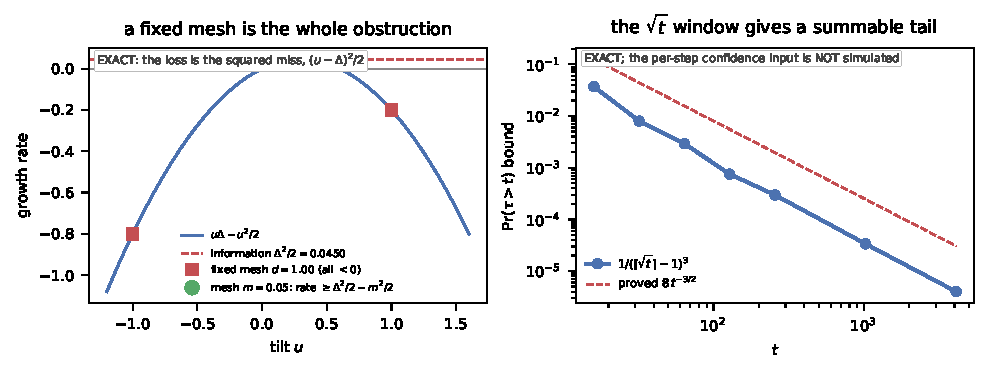
\includegraphics[width=\columnwidth]{paperA7_stopping_chain.pdf}
\caption{Left: at $\Delta=0.30$ the rate $u\Delta-u^{2}/2$ is negative at every non-zero
point of a fixed mesh $d=1$, while a mesh $m=0.05$ lands above $\Delta^{2}/2-m^{2}/2$ ---
the loss is the squared miss, so the fixed mesh is the whole obstruction. Right: at the
window $n=\lceil\sqrt t\,\rceil$ the failure mass $1/(n-1)^{3}$ sits under the proved
$8t^{-3/2}$, which is summable; the per-step confidence input is not simulated.}
\label{fig:a7chain}
\end{figure}
\begin{figure}[t]
\centering
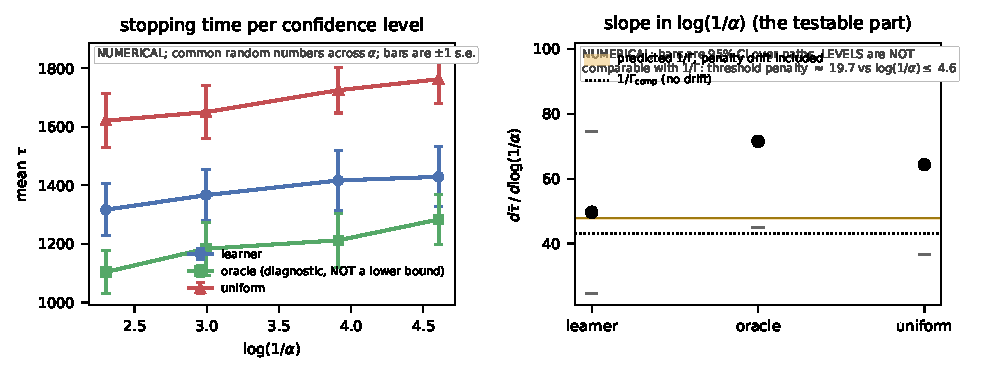
\includegraphics[width=\columnwidth]{paperA7_learner.pdf}
\caption{Left: stopping cost per unit of confidence for the three arms, against the
asymptotic \emph{bracket} for $1/\Gamma_{\rm comp}$. Right: every stopped run returned the
correct answer. Finite-$\alpha$ measurements; no ordering is asserted.}
\label{fig:learner}
\end{figure}

\begin{figure}[t]
\centering
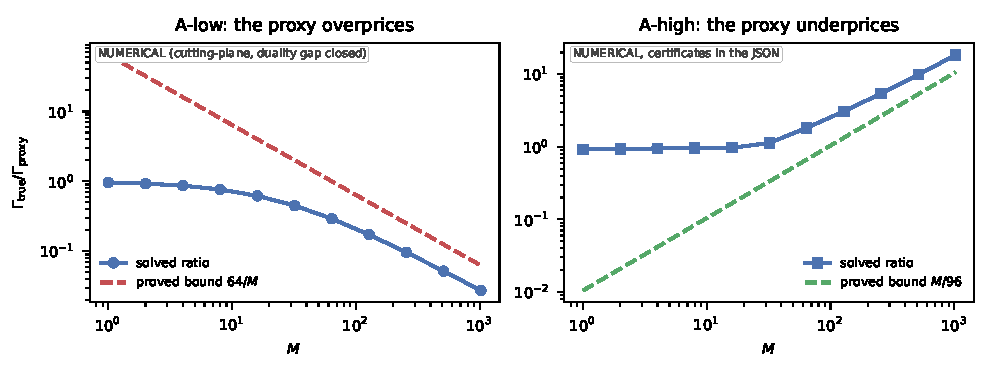
\includegraphics[width=\columnwidth]{paperA_separation_games.pdf}
\caption{The two optimised ratios against $M$, each with the bound
Theorem~\ref{thm:sep} proves. Cutting planes bracket both games; the brackets, not a single
number, are what is plotted.}
\label{fig:sepgames}
\end{figure}

\begin{figure}[t]
\centering
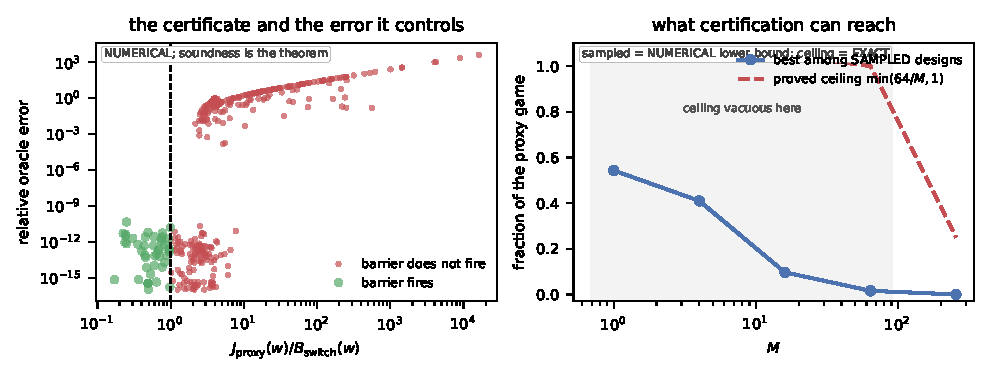
\includegraphics[width=\columnwidth]{paperA_repair_barrier.pdf}
\caption{Where the repair criterion fires, and the shaded band where the proved ceiling
$64/M$ exceeds $1$ and therefore says nothing.}
\label{fig:repair}
\end{figure}

\begin{figure}[t]
\centering
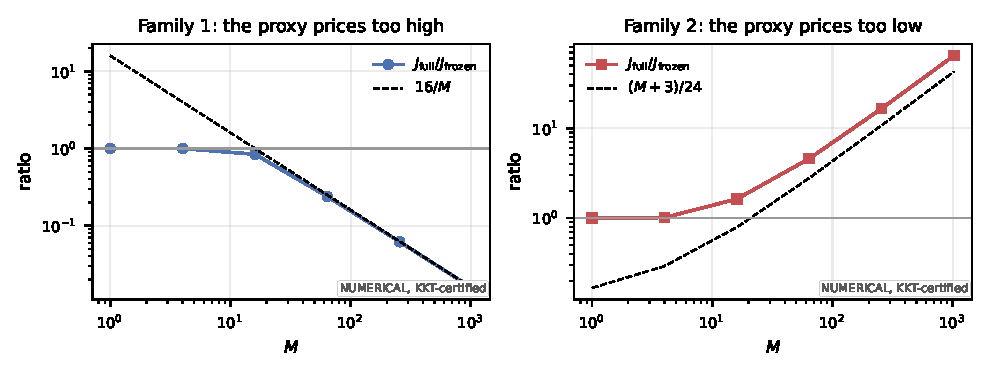
\includegraphics[width=\columnwidth]{paperA_frozen_proxy.pdf}
\caption{The surrogate misprices in both directions, against the predicted rates.}
\label{fig:proxy}
\end{figure}

\begin{figure}[t]
\centering
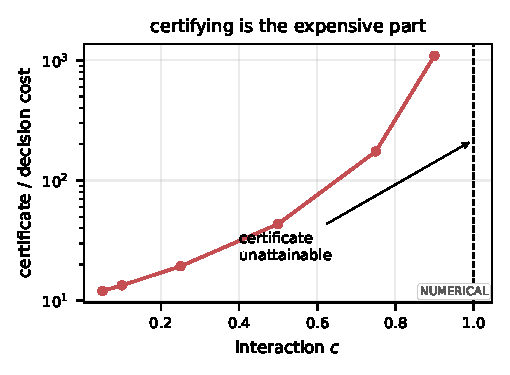
\includegraphics[width=0.78\columnwidth]{paperA_oracle_gap.pdf}
\caption{Certifying the margin against making the decision.}
\label{fig:margin}
\end{figure}

\section{Limitations}
\label{sec:limits}

\begin{enumerate}
\item[1)] \textbf{The two families are not yet realised in the model.} They are stated for a
range oracle with per-cell observations; the bridge of Section~\ref{sec:proxy} is owed.
\item[2)] \textbf{The certificates are numerical, not exact.} Every one of the $81$ regions
of every cell passes the KKT check, degenerate ones included: the multipliers are recovered
by \emph{non-negative} least squares, since on a region with linearly dependent active
constraints---one pinning the same index as both maximum and minimum---the minimum-norm
multipliers can be negative while admissible ones exist, and it is existence that
Theorem~\ref{thm:kkt} asks for. The residuals are floating-point, so this certifies
the decomposition to solver precision and not in exact arithmetic. A region that failed
would be reported and would fail the run's self-check, never dropped.
\item[3)] \textbf{The stopping analysis is conditional, not absent.} Section~\ref{sec:margin}
is an information-rate statement, and Section~\ref{sec:adaptive} now carries the whole
deterministic chain that converts it: accumulation on a good window, the derived event
inclusion, the union bound, the $\sqrt t$ window, the $t^{-3/2}$ tail, almost-sure
finiteness, and the $\limsup$. Its single remaining input is the per-step confidence
guarantee $\Pr(\text{fails at }s)\le s^{-4}$ for the algorithm's own statistic, which is a
Ville application not yet instantiated. The assembly step
$\mathbb{E}\tau\le t_{0}+\sum_{t\ge t_{0}}\Pr(\tau>t)$ is proved with no term discarded
(\lean{expectation\_le\_split} in \lean{LeanPaperClosuresV1}).
\item[4)] \textbf{The model is fixed, not derived} from the corpus definitions.
\item[5)] \textbf{Finitely many support points and competitors}, and nothing bounds the
number of regions, which is what decides whether enumeration is practical.
\end{enumerate}

\section{Conclusion}

The alternative set of a support-aware compression decision can be pinned exactly rather
than approximated, its regional minima and its design can both be certified rather than
searched, and the surrogate that freezes the extrema is wrong in both directions by
unbounded factors. Separately, certifying the margin that would justify a decision is up to
three orders of magnitude more expensive than the decision, and past a threshold impossible
while the decision stays easy. What remains owed is the bridge realising the two
counterexample families inside the linear model, and the one probabilistic input --- a
per-step confidence guarantee at level $s^{-4}$ --- that would make the stopping chain,
which is otherwise complete, turn an information-rate separation into a statement about
samples.

\section*{Companion material}
Two files accompany this paper and are part of the submission record.
\texttt{PROOFS.md} gives the central arguments as readable mathematics with no Lean
required --- setup, claim, proof, and in the same breath what the claim does not
cover. \texttt{DOSSIER.md} carries the full state: every audited theorem, every
measured number with its artifact and provenance status, the open list, and the
claims retracted during preparation, recorded rather than silently edited.
\texttt{CLAIMS.md} is the one-row-per-headline table of claim, final theorem,
remaining hypotheses and evidence.

\begin{thebibliography}{00}

\bibitem{schutte2026} N. Schutte et al., ``Sufficient decision proxies for
decision-focused learning,'' arXiv:2505.03953, 2026.

\bibitem{tosh2022} C. Tosh et al., ``Targeted active learning for probabilistic models,''
arXiv:2210.12122, 2022.


\bibitem{overstall2022} A. M. Overstall, ``Properties of Fisher information gain for
Bayesian design of experiments,'' Univ. of Southampton, 2022. [Online]. Available:
https://eprints.soton.ac.uk/452554/

\bibitem{filstroff2021} L. Filstroff, I. Sundin, P. Mikkola, A. Tiulpin, J. Kylm\"{a}oja,
and S. Kaski, ``Targeted active learning for Bayesian decision-making,'' arXiv:2106.04193,
2021.

\bibitem{tang2026} Y. Tang, S. Sloman, and S. Kaski, ``Error amplification under model
misspecification,'' in \emph{Proc. Machine Learning Research}, vol.~300, 2026.

\bibitem{bendavid2026} S. Ben-David and R. Kothari, ``A total function with randomized
query complexity quadratically below its certificate complexity,'' arXiv:2609.15063, 2026.

\bibitem{wan2026} Z. Wan, Y. Liu, P. Grigas, and Z.-J. M. Shen, ``Decision-focused
sequential experimental design,'' arXiv:2602.05340, 2026.


\bibitem{degenne2019} R. Degenne and W. M. Koolen, ``Pure exploration with multiple correct
answers,'' in \emph{Advances in Neural Information Processing Systems 32}, 2019,
pp.~14591--14600.

\bibitem{wangyou2026} Z. Wang and K. You, ``Information games with multiple correct answers
and piecewise-convex alternative sets,'' arXiv:2606.21889, 2026.

\bibitem{bennouna2026} A. Bennouna et al., ``Data informativeness in linear optimization,''
arXiv:2602.15365, 2026.

\bibitem{boyd2004} S. Boyd and L. Vandenberghe, \emph{Convex Optimization}. Cambridge,
U.K.: Cambridge Univ. Press, 2004.

\bibitem{pukelsheim2006} F. Pukelsheim, \emph{Optimal Design of Experiments}. Philadelphia,
PA: SIAM Classics in Applied Mathematics, 2006.

\bibitem{nitinawarat2013} S. Nitinawarat and V. V. Veeravalli, ``Controlled sensing for
sequential multihypothesis testing with controlled Markovian observations and non-uniform
control cost,'' \emph{Sequential Analysis}, vol.~34, no.~1, pp.~1--24, 2015.

\bibitem{mathlib2020} The mathlib Community, ``The Lean mathematical library,'' in
\emph{Proc. 9th ACM SIGPLAN Int. Conf. Certified Programs and Proofs (CPP)}, 2020,
pp.~367--381.

\bibitem{demoura2021} L. de Moura and S. Ullrich, ``The Lean 4 theorem prover and
programming language,'' in \emph{Proc. 28th Int. Conf. Automated Deduction (CADE)}, 2021,
pp.~625--635.

\end{thebibliography}

\end{document}
